\documentclass[a4paper,10pt]{scrartcl}

\usepackage{polski}
\usepackage[utf8]{inputenc}
\usepackage{graphicx}
\usepackage{enumerate}
\usepackage{pdflscape}

\title{Laboratorium 6}
\author{Filip Malinowski}
\date{\today}

\pdfinfo{%
  /Title    (Laboratorium 6)
  /Author   (Filip Malinowski)
}

\begin{document}

\title{Sprawozdanie z laboratorium 6}
\author{Filip Malinowski}
\date{\today}

\maketitle

Do programu zostały dodane lista asocjacyjna
oraz tablica z haszowaniem.

Lista asocjacyjna jest odpowiednikiem tablicy
asocjacyjnej wykonanej na liście. Do listy
dodałem podstawowe metody do wstawiania pary
klucz-wartość, do usuwania wszystkich elementow
z listy, itd.

W tablicy z haszowaniem wybrałem haszowanie
wzorowane na kukułczym. Zastosowałem do tego
dwie tablice przechowujące pary klucz-wartość.
Lewa tablica korzysta z funkcji haszującej
Shift-Add-XOR. Prawa tablica korzysta z
Fowler/Noll/Vo.
Wybrałem ten typ tablicy z haszowaniem
ze względu na teoretycznie wyższą szybkość
działania w porównaniu do wstawiania
progresywnego przy wystąpieniu konfliktu.
Różni się to od haszowania kukułczego tym,
że nie losuję tutaj funkcji haszujących
tylko korzystam z dwóch predefiniowanych.

\pagebreak

Implementacje sortowania przeniosłem z programu
Szymona Furmańczyka do swojego z racji tego, że
łatwiej mi było zautomatyzować badanie czasu
sortowania.

W klasie Stos są teraz sortowania szybkie, przez
scalanie i przez kopcowanie. Quicksort jest napisany
w dwóch wersjach. Pierwsza, w której pivot pobierany
jest z początku listy tablicowej. Druga w której 
pivot to średnia trzech elementów: z początku,
środka i końca stosu.

Z otrzymanych danych można wywnioskować, że moja implementacja
quicksort działa o wiele szybciej dla dużej ilości danych 
niż sortowanie przez kopcowanie. Natomiast po optymalizacji
quicksort sortował wolniej dla małej ilości danych niż przed
optymalizacją. Po optymalizacji pivota czas sortowania jest
podobny do czasu sortowania bez optymalizacji.
Dla drugiego zestawu danych wejściowych quicksort bez optymalizacji
działał już 6 razy wolniej dla 100 000 elementów niż po optymalizacji.

Sortowanie przez kopcowanie ma dość wolny czas działania.
Najwolniejszy z trzech napisanych przeze mnie sortowań.
Implementację napisałem na nowo starając się napisać szybsze
sortowanie.

Sortowanie przez scalanie ma stałą złożoność obliczeniową
w każdym przypadku danych wejściowych (posortowanych
lub nie). Wynika to z działania algorytmu i zostało
sprawdzone doświadczalnie podczas pomiarów.
Podczas sortowania danych wstępnie posortowanych
mergesort sortował wyraźnie szybciej niż
quicksort po optymalizacji dla 100 i 1000 elementów
Dla 10 000 i 100 000 sortował już wolniej.
Można więc napisać sortowanie hybrydowe, które
uruchamiałoby mergesort dla małej ilość danych
wejściowych do sortowania, a powyżej pewnego
progu (w tym przypadku 10 000 elemtów) uruchamiałoby
quicksort. Można w ten sposób skorzystać z
dobrych stron obu sortowań w jednym.

\pagebreak

\begin{landscape}
\begin{figure}
 \centering
  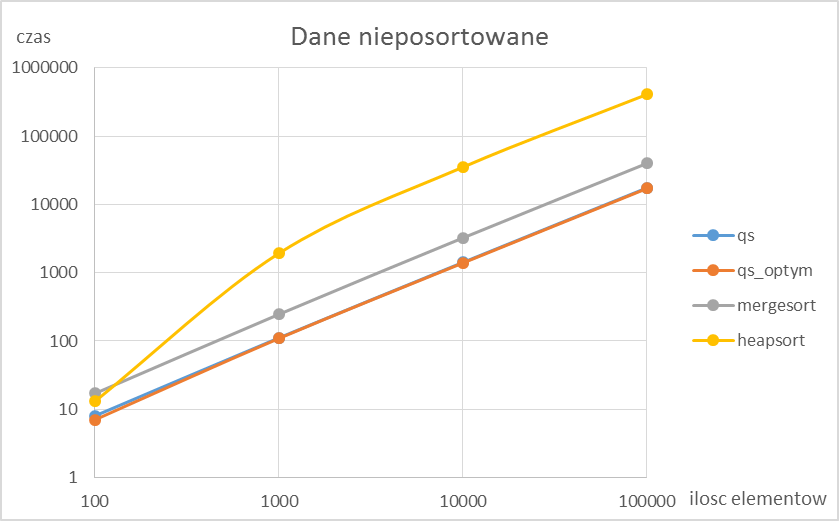
\includegraphics[scale=1]{wyk1}
 \caption{Czas sortowania elementów dla danych nieposortowanych}
\end{figure}

\pagebreak

\begin{figure}
 \centering
  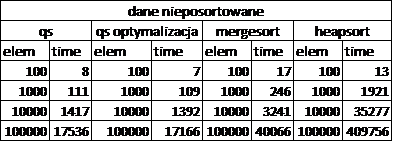
\includegraphics[scale=1]{tab1}
 \caption{Tabela z wartościami pomiarowymi}
\end{figure}

\begin{figure}
 \centering
  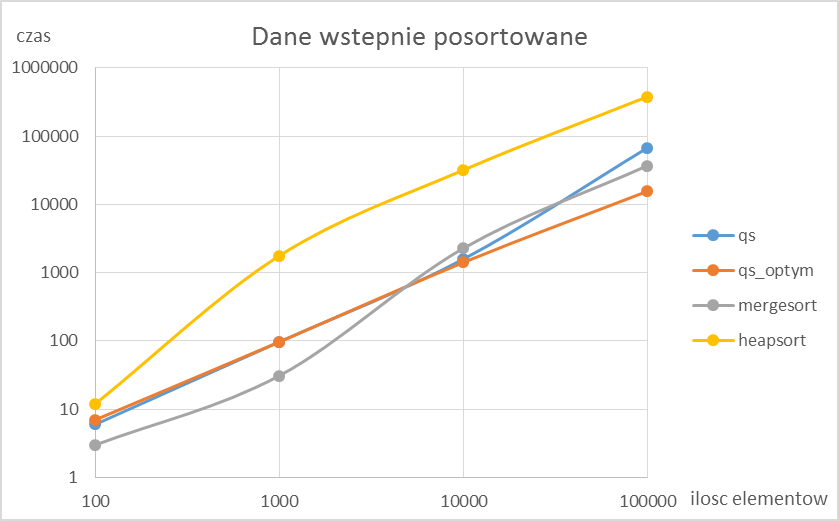
\includegraphics[scale=1]{wyk2}
 \caption{Czas sortowania elementów dla danych wstępnie posortowanych}
\end{figure}

\pagebreak

\begin{figure}
 \centering
  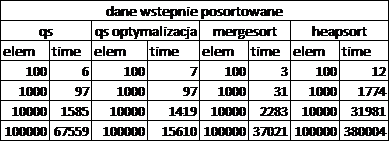
\includegraphics[scale=1]{tab2}
 \caption{Tabela z wartościami pomiarowymi}
\end{figure}
\end{landscape}

\end{document}
